\en{
\section{General Information}
\subsection{Architektur}
This app uses the Model View ViewModel (MVVM) architecture, which is a common architecture, splitting the software into three layers:
\begin{itemize}
	\item \textbf{The Model} contains the data, which can be modified by the ViewModel. The data is independent of the other layers, meaning multiple views implementations can use the same model. It might also contain some business logic, like accessing the devices main memory. For this project, the Models will be called XYZState.
	\item \textbf{The ViewModel} takes user inputs from the View and modifies the models data accordingly. It also iffer the view access to the state of the model, so any changes can be reflected in the UI. For this project, the View Models will be called XYZViewModel, with event that can happen being called XYZEvent.
	\item \textbf{The View} reacts to changes in the ViewModel and reflects those changes in the UI. It should contain no business logic. For this project, the Views will be called XYZScreen.
\end{itemize}
This architecture was used as the apps UI used Jetpack Compose, which is made to work with a ViewModel. The separation of the layers also allows for independent changes between UI and business logic, as well as bester testability, as no complex UI tests are needed to test the business logic.

\subsubsection{Data Bindings}
For databindings, Jetpack Compose already provides states that take care of updating and recomposing the UI.

\subsubsection{Further Resources}
\href{https://www.youtube.com/watch?v=8YPXv7xKh2w}{This YouTube video} further explains the MVVM architecture and was used by the developers of this app to learn it.

}


\de{
\section{Allgemeine Informationen}
\subsection{Architektur}
Diese App nutzt die Model View ViewModel Architektur, eine weiterverbreite Architektur, welche die Software in drei Schichten unterteilt:
\begin{itemize}
	\item \textbf{Das Model} enthält die Daten, die vom ViewModel modifiziert werden können.  Die Daten des Models sind unabhängig von den anderen Schichten und können daher von unterschiedlichen View Implementierungen verwendet werden. Es kann auch Geschäftslogik in dem Model liegen, wie das Einlesen von Daten aus dem Speicher.
	\item \textbf{Das ViewModel} nehmen Eingaben der UI über den View entgegen und modifizieren ggf. die Daten des Models. Sie bieten dem View einen State des Models, sodass die UI bei einer Änderung dieses States angepasst werden kann.
	\item \textbf{Der View} reagiert auf Änderungen des ViewModels und stellt diese in der UI da. Der View enthält keine Geschäftslogik.
\end{itemize}
Diese Architektur wird verwendet, da die UI der App mit Jetpack Compose entwickelt wurde, welches auf die Verwendung mit einem ViewModel ausgelegt ist. Des weiteren erlaubt die klare Trennung der Schichten eine unabhängige Entwicklung von UI und Geschäftslogik und erlaubt ein testen der Geschäftslogik ohne komplexe UI Tests.



\subsubsection{Datenverbindungen}
Jetpack Compose kommt bereits mit fertigen Datenverbindungen, welche dafür sorgen das UI und Model entsprechend der Änderungen angepasst werden.

\subsubsection{Weitere Ressourcen}
\href{https://www.youtube.com/watch?v=8YPXv7xKh2w}{Dieses Youtube Video} erklärt die MVVM Architektur im Detail und wurde von den Entwicklern dieser App verwendet, um die Architektur zu lernen.
}

\begin{figure}[H]
	\centering
	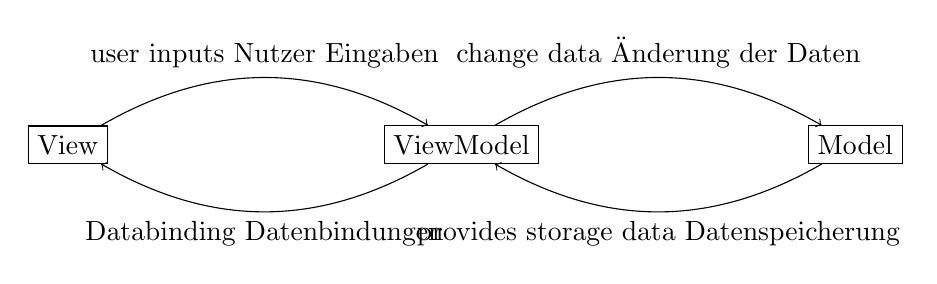
\begin{tikzpicture}[node distance=5cm]
		% Nodes
		\node (View) [draw, rectangle] {View};
		\node (ViewModel) [draw, rectangle, right of = View] {ViewModel};
		\node (Model) [draw, rectangle, right of = ViewModel] {Model};
		
		% Arrows
		\draw[->] (View) to[bend left] node[midway, above] {\en{user inputs} \de{Nutzer Eingaben}} (ViewModel) ;
		\draw[<-] (View) to[bend right] node[midway, below] {\en{Databinding} \de{Datenbindungen}} (ViewModel) ;
		\draw[->] (ViewModel) to[bend left] node[midway, above] {\en{change data} \de{Änderung der Daten}} (Model) ;
		\draw[<-] (ViewModel) to[bend right] node[midway, below] {\en{provides storage data} \de{Datenspeicherung}} (Model) ;
	\end{tikzpicture}
	\caption{\en{Overview of the MVVM architecture} \de{Überblick über die MVVM Architektur}}
	\label{fig:MVVM}
\end{figure}